%%%%%%%% ICML WORKSHOP SUBMISSION %%%%%%%%
\documentclass{article}
\usepackage{microtype}
\usepackage{graphicx}
\usepackage{booktabs}
\usepackage{hyperref}
\usepackage{amsmath}
\usepackage{amssymb}
\usepackage{amsthm}
\usepackage{mathtools}
\usepackage{multirow}

\usepackage[accepted]{icml2025}
\usepackage[capitalize,noabbrev]{cleveref}

% The template loads times.sty, whose bold face is absent from this TeX
% bundle, so every \bf / \bfseries silently fell back to regular weight.
% newtxtext supplies a real Times bold; \bf is also restored for the
% template's LaTeX 2.09-era heading macros.
\usepackage{newtxtext}
\makeatletter
\let\bf\bfseries
\makeatother

\newtheorem{theorem}{Theorem}

\icmltitlerunning{PDE Spheroid Modeling for Probabilistic Drug Search}

\setcounter{topnumber}{3}
\setcounter{totalnumber}{4}
\renewcommand{\topfraction}{0.9}
\renewcommand{\textfraction}{0.07}
\renewcommand{\floatpagefraction}{0.75}

\begin{document}

% The style file's running-head guard tests \ht of a \vbox against 6.25pt;
% with this build's font metrics even a one-line title measures 6.35pt, so the
% guard trips and substitutes its placeholder. Restore the intended header.
\makeatletter
\let\ps@icmlorig\ps@fancy
\makeatother

\twocolumn[
\icmltitle{PDE Reaction--Diffusion Spheroid Modeling\\
for Probabilistic Chemotherapy Drug Search}

\begin{icmlauthorlist}
\icmlauthor{Ishan Gonehal}{ind}
\end{icmlauthorlist}
\icmlaffiliation{ind}{Independent Researcher}
\icmlcorrespondingauthor{Ishan Gonehal}{ishangonehal@berkeley.edu}

\icmlkeywords{Bayesian optimization, combinatorial pools, structured kernels,
drug combinations, reaction--diffusion}

\vskip 0.3in
]

\printAffiliationsAndNotice{Presented at the Structured Probabilistic Inference
\& Generative Modeling workshop (SPIGM) at ICML 2026.}

\chead{\small\bfseries PDE Spheroid Modeling for Probabilistic Drug Search}

\begin{abstract}
Bayesian optimization (BO) over finite combinatorial pools is scored, almost
universally, by a single scalar measured in a well-mixed monolayer assay.
Savitar, a curve-aware interaction-structured kernel, attains the lowest mean
regret on such pools by converting per-constituent response curves into
activity-gated embeddings coupled through a shared low-rank tensor
factorization. Part~I condenses that method and its cross-domain evidence.
Part~II asks a question the original evaluation cannot: whether the
combinations a curve-aware optimizer selects remain the best ones once
\emph{space} is modeled. We simulate the selections of sixteen BO methods on
the NCI-ALMANAC panel~\citep{holbeck2017} in a spatially resolved spheroid
reaction--diffusion model with oxygen-limited proliferation, hypoxic
resistance, and finite drug transport. The well-mixed ODE bridge used
previously is exactly rank-preserving (Spearman $\rho = -1.0000$); the
spheroid is not ($\rho = -0.56$, with $36.5\%$ of within-cell-line pairs
re-ordered). In vitro potency explains $23\%$ of the variance in spheroid
outcome; one spatial quantity raises this to $86\%$. Savitar keeps a large
advantage over every structural baseline but places fifth of sixteen on
spheroid log-kill AUC, and the deficit is mechanistic: outcome tracks
residual hypoxic fraction ($\rho = -0.969$) more tightly than potency
($\rho = -0.767$), and Savitar selects combinations $7.5$ percentage points
\emph{more} potent in vitro that leave $62\%$ more hypoxic tissue.
Combination BO should be scored on spatially resolved, outcome-anchored
readouts.
\end{abstract}

\section{Introduction}

Drug-combination screening, phase-specific alloy design, and same-day options
strategy search are not usually thought of as the same problem, but each is a
search over a finite, enumerable pool under a budget that is a small fraction
of pool size, with a long-tailed value distribution in which a tiny minority
of candidates are useful, and each is paired with prior information that
practitioners routinely measure before any combination is queried. Bayesian
optimization (BO) is the standard framework for such budgets, yet
off-the-shelf kernels (Mat\'ern on raw descriptors, Hamming on identities,
Tanimoto on fingerprints) discard the richest available structure: the
\emph{per-constituent response curve} (the dose--response curve, the unary
phase-boundary curve, the implied-volatility smile). These curves are
informative about how each constituent behaves in combination, cheap to
obtain, and shared across every combination containing that constituent.

Part~I condenses Savitar~\citep{gonehal2026savitar}, a structured GP kernel that consumes the curve
directly through two priors: an \emph{activity gate} vanishing when a
constituent is inactive at its operating point, and a \emph{symmetric
CP-tensor parameterization} sharing interaction parameters across all subset
orders, reducing the effective parameter count to $O(Dq)$ regardless of
arity and letting few observations generalize across unseen combinations.
It is a drop-in kernel replacement requiring no new acquisition machinery.
This material is published work, included as the foundation the extension
builds on.

Part~II is new. Every result in Part~I, and in the combination-BO literature
generally, is scored on a number measured in a well-mixed monolayer: percent
growth inhibition at a fixed exposure. That number is what the optimizer
maximizes and what benchmark regret is computed from. It is also blind to
\emph{where} in a tumor the killing happens. We build a spatially resolved
spheroid reaction--diffusion model, re-score the selections of sixteen BO
methods under it, and find the method ranking changes, for reasons that are
mechanistically identifiable and that suggest a concrete extension to the
kernel itself.

\section{Related Work}

Neural combination surrogates reach strong retrospective accuracy on
$10^4$--$10^5$ labeled triples, but sequential discovery operates in the
opposite regime ($\le 30$ evaluations against $10^4+$ candidates) where
deep surrogates have poorly calibrated uncertainty. Combinatorial and
discrete BO innovate on acquisition or search geometry (COMBO's graph
Cartesian product, BOCS's sparse binary regression, trust-region methods);
Savitar attacks the kernel side instead, consuming the per-constituent curve
as a structured prior rather than relearning it. Among set-function and
tensor-structured kernels, DeepSets~\citep{zaheer2017} learns set functions without an activity
gate or CP coupling and SAAS~\citep{eriksson2021} is a sparsity-aware GP; CP decompositions~\citep{bro1997} appear
in multi-output GPs and collaborative filtering. Savitar combines CP
interaction weights with activity-gated embeddings for finite-pool discovery.
Reaction--diffusion models of avascular spheroids with oxygen-limited
proliferation are long established as descriptions of viable-rim/hypoxic/
necrotic layering; to our knowledge they have not previously been used as an
\emph{evaluation instrument} for combination-selection algorithms, which is
the use we make of one here.

\section{Method}
\label{sec:method}


\paragraph{The pipeline at a glance.} The shared input across domains is a
finite candidate pool together with the per-constituent response curves that
domain practitioners measure before any combination is queried. The paradigm
pipeline feeds constituent identities (and, optionally, chemistry-derived
fingerprints) to a generic Hamming or Tanimoto kernel, discarding the curve
information entirely; the resulting similarity kernel treats every pair of
identical constituents the same regardless of where on the dose--response or
phase-boundary curve they sit. Savitar instead consumes each curve through an
activity-gated linear projection that produces a per-constituent embedding
$f_i$, then aggregates across constituents through a symmetric CP-tensor
parameterization that shares interaction parameters $A$ across all subset
sizes. The output is a single feature vector $\phi(c) \in \mathbb{R}^q$ on
which a Gaussian RBF kernel is computed. The GP posterior on the unobserved
pool, scored by Expected Improvement, picks the next query, and the loop
repeats until the budget is exhausted.

\subsection{Problem formulation}

A combinatorial discovery problem is a triple $(\mathcal{C}, f, T)$: a finite
candidate pool $\mathcal{C}$ of size $P$, an oracle $f: \mathcal{C} \to
\mathbb{R}$ returning a scalar quality value when queried, and a budget
$T \ll P$ of permitted queries. Each candidate is a tuple
$c = (i_1,\ldots,i_k; d_1,\ldots,d_k)$ of $k$ constituent identities
$i_j \in [D]$ and corresponding operating points $d_j \in \mathbb{R}$. The
objective is to find $c^\star \in \arg\min_{c \in \mathcal{C}} f(c)$ within
$T$ queries; performance is reported as final regret
$|f(c_T) - f(c^\star)|$. This abstraction covers drugs at log-doses against a
cell-line oracle ($D \approx 100$, $k = 2$, $P \approx 4.5 \times 10^4$);
elements at mole fractions against a phase-equilibrium oracle; and option
contracts at quantities against a one-day P\&L oracle. The four properties
that recur and motivate Savitar's design are: pools are finite and
enumerable, budgets are small fractions of $P$, high-value candidates are
rare, and each constituent admits an individual-response curve fit upstream
of any combination measurement.

\subsection{Per-constituent fingerprints}

For each constituent $i$ in a given context we fit a fixed parametric model
to its individual-response data and store the parameter vector
$e_{i,c} \in \mathbb{R}^p$ as a fingerprint. The choice of curve family is a
domain question (Hill, polynomial, implied-volatility smile); $p$ is small,
typically four or five. The fingerprint admits a deterministic readout
$\mathrm{curve}(d; e_i) \to \mathbb{R}$, and we define the \emph{activity}
\begin{equation}
s_i = \mathrm{clip}\!\left(\tfrac{1}{R}\,\mathrm{curve}(d_i; e_i),\, 0,\, 1\right) \in [0,1],
\end{equation}
where $R$ is a domain-specific normalizing scale ($R = 100$ for percent
growth). The parameter vector itself is an information-rich summary of how the
constituent will respond at any operating point, not just at $d_i$; we
$z$-score $e_{i,c}$ within a context to put every curve parameter on the same
scale and write $e_i^z$ for the result. The curve resolves how a constituent
behaves in isolation; combination-specific effects must be modeled
separately, which is the role of the CP-tensor structure.

\subsection{From a naive curve embedding to the activity gate}

The simplest way to put curve information into a kernel is to project the
$z$-scored fingerprint as $f_i = M e_i^z$ through a learnable linear map
$M \in \mathbb{R}^{q \times p}$ (this baseline is exactly the
\textsc{linear\_curve} surrogate, which already accounts for a fraction of
Savitar's improvement). It is missing one piece of structure.

\paragraph{The vanishing constraint.} A synergistic combination $S$ should
not contribute to the GP feature when any constituent $i_j$ in $S$ is
operated at its no-effect point. Bliss-style independence formalizes this:
an interaction term is informative only when all participating constituents
are active. Let $g: [0,1] \to [0,1]$ be a smooth monotonic gate applied to
the activity $s_i$ and consider the interaction feature
\begin{equation}
\bigodot_{j \in S} f_{i_j}
 = \prod_{j \in S} g(s_{i_j}) \bigodot_{j \in S} M e_{i_j}^z .
\end{equation}
For the right-hand side to vanish when any single constituent in $S$ is
inactive ($s_{i_j} = 1$), the factor $\prod_j g(s_{i_j})$ must equal zero,
forcing $g(1) = 0$. Symmetrically, the interaction should be maximal when
every constituent is fully active ($s_{i_j} = 0$), i.e.\ $g(0) = 1$. Among smooth monotonic functions on $[0,1]$ satisfying these endpoints, $g(s) = 1 - s$ is the unique linear choice and the simplest non-trivial member of the family $g(s) = (1-s)^\alpha$.

\paragraph{Activity-gated embedding.} We adopt $g(s) = 1 - s$ throughout:
\begin{equation}
f_i = (1 - s_i)\cdot M e_i^z \in \mathbb{R}^q .
\label{eq:gate}
\end{equation}
The factor $(1 - s_i)$ has a direct domain reading in each application (the
per-drug kill fraction in pharmacology, the fractional saturation in
chemistry, the moneyness-adjusted leg activation in options), and it makes
the no-effect-vanishing property automatic for all higher-order interactions.

\subsection{Symmetric CP sharing}

The most general parameterization of a symmetric order-$m$ interaction over
$D$ constituents is a symmetric tensor $T^{(m)}$ with
$\binom{D+m-1}{m}$ free parameters: for $D = 100$ and $m = 3$ that is
$1.7 \times 10^5$, more than the entire ALMANAC pool for any single cell
line, with at most $T \le 30$ observations to fit it. A rank-$q$ symmetric CP
decomposition instead gives
\begin{equation}
T^{(m)}_{i_1 \cdots i_m} = \sum_{r=1}^{q} \prod_{j=1}^{m} A[i_j, r],
\qquad A \in \mathbb{R}^{D \times q},
\label{eq:cp}
\end{equation}
introducing $Dq$ parameters regardless of $m_{\max}$ and arity $k$. For
$D = 100$, $q = 8$ this is $800$ parameters, comfortably below budget.
Crucially, the same row $A[i,:]$ is reused for every order, which is the
mechanism by which an observation at any combination involving $i$ propagates
to every other combination involving $i$.

\subsection{Aggregation, kernel, and BO loop}

The Hadamard product $\bigodot_{j \in S} f_{i_j} \in \mathbb{R}^q$ preserves
both multiplication and dimension. Combining \cref{eq:gate,eq:cp} gives
\begin{equation}
\phi(c) = \sum_{j=1}^{k} f_{i_j}
 + \sum_{m=2}^{m_{\max}} \sum_{\substack{S \subseteq [k] \\ |S| = m}}
 w_S \cdot \bigodot_{j \in S} f_{i_j} \in \mathbb{R}^q ,
\end{equation}
with $w_S = \sum_r \prod_{j \in S} A[i_j, r]$. The activity gate factors out
of every order-$m$ term as $\prod_{j \in S}(1 - s_{i_j})$, so a synergistic
interaction contributes feature mass only when every constituent in $S$ is
individually active. The final kernel is a radial basis function on $\phi$:
\begin{equation}
k(c, c') = \sigma^2 \exp\!\left(-\tfrac{1}{2\ell^2}\|\phi(c) - \phi(c')\|^2\right),
\label{eq:rbf}
\end{equation}
with learnable signal variance $\sigma^2$ and lengthscale $\ell$. Since
$\phi$ is deterministic given $(M, A)$, $k$ is the Gaussian RBF composed with
a feature map and is therefore PSD on $\mathcal{C}$.

Cross-combination generalization follows: an observation at any combination
containing constituent $i$ propagates to the posterior at every other
combination containing $i$, including unseen pairs and triplets, because
$\partial\phi(c)/\partial A[i,:] \ne 0$ generically. \Cref{app:proof} states
and proves this.


\paragraph{BO loop.} At step $t$ we refit
$\theta = \{M, A, \ell, \sigma^2, \sigma_n^2\}$ on the observations by
Type-II marginal-likelihood maximization (30 Adam steps at lr $0.05$), score
each unobserved $c$ by Expected Improvement, and query the argmax. The
dominant cost is the Adam fit at ${\sim}0.03$\,s per step on CPU; end-to-end
this yields a ${\sim}0.9$\,s BO trajectory on ALMANAC, 2--10$\times$ faster
than published GP baselines.

\begin{table*}[t]
\caption{Cross-domain final regret (mean over seeds) for every method in the Part~I evaluation,
reproduced from the predecessor paper~\citep{gonehal2026savitar}. Bold is best per column; en dashes mark domain-inapplicable
cells. Under a single fixed hyperparameter configuration, Savitar attains the lowest mean regret on
eight of the ten primary benchmarks, losing Tan/HIV to \texttt{linear\_curve} and Ni$_3$Zn$_{14}$ to
\texttt{saas}. Two patterns matter for Part~II. First, the margin is largest exactly where the pool
is large and winners are rare (ALMANAC, $5.54$ against $9.16$ for the strongest curve baseline and
$70.4$ for random), and it narrows or inverts on the small chemistry pools where a sparsity prior
has less to overcome; this is the regime characterization Part~II inherits when it restricts to
in-regime cell lines. Second, the ablations locate the gain: removing the activity gate
(\texttt{savitar\_no\_gate}) costs an order of magnitude on ALMANAC ($82.2$) and on Cokol
($0.838$ against $0.018$), whereas removing higher-order interaction terms (\texttt{savitar\_no\_m})
is nearly free on the small pools and even wins three columns, so the gate carries the
combinatorial-scale win and the tensor carries the interaction structure. Every number here is
scored on well-mixed in vitro regret, the single scalar whose sufficiency Part~II tests.}
\label{tab:crossdomain}
\vskip 0.1in
\centering
\scriptsize
\setlength{\tabcolsep}{3.2pt}
\begin{tabular}{l cccc ccc ccc}
\toprule
& \multicolumn{4}{c}{Drug discovery} & \multicolumn{3}{c}{Chemistry (Ni--Sn--Zn)} & \multicolumn{3}{c}{Finance (ETF options)} \\
\cmidrule(lr){2-5}\cmidrule(lr){6-8}\cmidrule(lr){9-11}
Method & ALMANAC & Cokol & Tan/HIV & Brochado & Ni$_3$Zn$_{14}$ & Sn & Ni$_3$Sn-HT & ETF fam. & SPY mo. & QQQ mo. \\
\midrule
\multicolumn{11}{l}{\emph{Random and identity-only baselines}}\\
random & 70.4 & 0.51 & 9.32 & 6.18 & .019 & .008 & .020 & .560 & .373 & 1.12 \\
hamming & 56.2 & -- & -- & -- & -- & -- & -- & -- & -- & -- \\
act\_hamming & 56.2 & -- & -- & -- & -- & -- & -- & -- & -- & -- \\
\multicolumn{11}{l}{\emph{Published domain-aware baselines}}\\
tanimoto & 79.1 & -- & 13.45 & -- & -- & -- & -- & -- & -- & -- \\
gip & -- & 0.73 & -- & -- & -- & -- & -- & -- & -- & -- \\
chemogenomic & -- & -- & -- & 3.30 & -- & -- & -- & -- & -- & -- \\
\multicolumn{11}{l}{\emph{Flat / curve-aware GP baselines}}\\
flat\_matern\_id & 81.8 & -- & -- & -- & -- & -- & -- & -- & -- & -- \\
flat\_matern\_curve & 90.6 & 1.65 & 12.18 & 3.60 & .024 & .006 & .018 & -- & -- & -- \\
linear\_curve & 9.16 & 0.020 & \textbf{2.65} & 1.25 & .019 & .0024 & .0038 & -- & -- & -- \\
sphere\_linear\_curve & 32.7 & -- & -- & -- & -- & -- & -- & -- & -- & -- \\
linear\_descriptor & -- & -- & -- & -- & -- & -- & -- & .339 & .285 & .502 \\
linear\_option\_curve & -- & -- & -- & -- & -- & -- & -- & .070 & .075 & .058 \\
\multicolumn{11}{l}{\emph{Learned and set-function baselines}}\\
deep\_ensemble & 15.2 & 0.084 & 7.41 & 2.39 & .019 & .0029 & .0044 & .147 & .110 & .261 \\
deepsets & 13.3 & 0.247 & 8.16 & 7.76 & .016 & .008 & .020 & -- & -- & -- \\
saas & -- & -- & -- & -- & \textbf{.013} & .0041 & .009 & -- & -- & -- \\
\multicolumn{11}{l}{\emph{Savitar structural ablations}}\\
savitar\_no\_m & 6.28 & \textbf{.014} & 13.86 & 1.15 & .021 & .0011 & .024 & \textbf{.045} & \textbf{.060} & \textbf{.000} \\
savitar\_no\_gate & 82.2 & 0.838 & 14.52 & 0.57 & .026 & \textbf{.0004} & .013 & .046 & .061 & \textbf{.000} \\
\multicolumn{11}{l}{\emph{Savitar (full)}}\\
\textbf{savitar} & \textbf{5.54} & .018 & 5.43 & \textbf{.040} & .017 & .0017 & \textbf{.0033} & .048 & .064 & \textbf{.000} \\
\bottomrule
\end{tabular}
\vskip -0.1in
\end{table*}

\section{Cross-Domain Evaluation and Regime Boundaries}
\label{sec:experiments}
\label{sec:regimes}

Table~\ref{tab:crossdomain} gives the full cross-domain result.
Savitar is evaluated on three domains under one fixed configuration
($q = 8$, $m_{\max} = 2$, ZeroMean, 30 Adam steps at lr $0.05$) with no
per-domain retuning, against random search, identity kernels (Hamming,
activity-Hamming), each field's published domain kernel (Tanimoto, GIP,
INDIGO chemogenomic), flat and curve-aware Mat\'ern GPs, deep ensembles,
DeepSets, SAAS, and its own two structural ablations. In \emph{drug
discovery} it wins clearly where one drug's effect depends on what another
is doing (Brochado, an order of magnitude below the curve-aware baselines),
ties the linear baseline where the dose--response signal is already strong
(Cokol), improves $1.8\times$ on the chemistry-aware Tanimoto kernel on the
legacy NCI-60 sweep, and is overtaken on Tan/HIV where the curve alone
explains the data. In \emph{chemistry} (Ni--Sn--Zn phase equilibria) SAAS
narrowly wins the one phase with the fewest participating elements while
Savitar beats every method on the two with more. In \emph{finance}
(same-day ETF options) its lead over the curve-only baseline widens as
profitable strategies get rarer ($0.0476$ vs.\ $0.0703$, $p = 0.0019$).

\paragraph{What carries the win, and where it stops.} The two ablations are
diagnostic and complementary: fixing $M = I_4$ ties full Savitar on Cokol
but degrades badly on Brochado, while removing the activity gate is
catastrophic on Cokol and mild on Brochado, so each contribution carries the
win where the other is weakest. A capacity sweep finds $q \in \{4,8\}$
optimal everywhere, so the benefit is the presence of structured interaction
sharing rather than its capacity. The cells where Savitar is \emph{not} best
each violate one of the four regime properties: MOLT-4 has $6.7\%$ of its
pool within regret 5 of the optimum, so random search already finds it; on
Tan/HIV and on the ALMANAC representative subset the per-constituent signal
is dense enough that the linear curve baseline wins; on the smallest alloy
phase the sparse axis-aligned prior wins. These are not failure
modes but predictions of when the inductive bias should and should not
help, and Part~II takes that regime-dependence seriously, deriving its
analysis cohort from the near-optimum-density criterion rather than assuming
uniform applicability.

\section{Justifying Rescoring}
\label{sec:pde-intro}

Every number in Part~I is a scalar measured in a well-mixed monolayer:
percent growth inhibition at a fixed exposure and time. That number is what
the optimizer maximizes and what regret is computed from. A solid tumor is
not well mixed: drug arrives by diffusion, oxygen falls off over
${\sim}150$--$200\,\mu$m, and cells in the resulting hypoxic interior divide
slowly and resist cycle-dependent agents. A combination potent in a monolayer
may or may not clear that interior.

The predecessor work~\citep{gonehal2026savitar} anticipated the need for a pharmacological bridge and
supplied one: Gompertz growth with linear PK, converting the BO objective
into a simulated tumor burden. That bridge is well-mixed by construction, and
we show in \cref{sec:ode} that it is \emph{exactly} rank-preserving: it
cannot change which combination looks better, only restate the in vitro
number on another scale. To ask whether spatial structure changes the answer,
the model must have space in it.

\section{Spatial Model and Readouts}

\subsection{Analysis cohort and the out-of-regime control}
\label{sec:cohort}

Part~I documents where curve-aware selection does and does not help, and the
governing quantity is \emph{near-optimum density}: the fraction of the pool
within a small regret of the optimum. Where that fraction is large, random
search already succeeds and no prior can add much. We therefore derive the
cohort from the data rather than copying a list: recomputing near-optimum
density for all 60 ALMANAC cell lines reproduces the two values the
predecessor paper~\citep{gonehal2026savitar} reports (OVCAR-8 at $0.00046$ against a published $0.05\%$;
MOLT-4 at $0.0676$ against $6.7\%$), and a threshold of $0.005$ places 50 of
60 cell lines in regime. Applied blind to the eight cell lines of the
predecessor's ALMANAC study, it admits exactly seven and excludes exactly
MOLT-4, the line that paper itself names as out of regime.

The seven in-regime lines (DU-145, HT29, OVCAR-8, MDA-MB-231/ATCC,
MDA-MB-435, PC-3, T-47D) form the analysis cohort; MOLT-4 is retained as a
labelled out-of-regime control (\cref{sec:molt4}). The split is not
cosmetic: curve-aware selection beats the structural baseline on $45/50$
in-regime lines versus $5/10$ out of regime (Fisher $p = 0.0078$,
OR $= 9.0$).

\subsection{Spheroid reaction--diffusion model}
\label{sec:model}

We model a radially symmetric spheroid of radius $R = 400\,\mu$m. The state
is viable cell density $n(r,t)$, oxygen $c_O(r,t)$, and one field
$c_j(r,t)$ per drug in EC50 multiples:
\begin{align}
\partial_t n ={}& D_n \nabla^2 n
 + \rho\, n (1-n) \tfrac{c_O}{K_O + c_O} \nonumber\\
 &- \delta_{\text{hyp}} n \mathbf{1}[c_O < \theta]
 - K(c, c_O)\, n \\
0 ={}& D_O \nabla^2 c_O - q_O\, n \tfrac{c_O}{K_O + c_O} \\
\partial_t c_j ={}& D_j \nabla^2 c_j
 - u_j n \tfrac{c_j}{K_u + c_j} - \lambda_j c_j
\end{align}
Each drug contributes a Hill-form kill rate from its fitted monotherapy
curve; drugs combine additively (Bliss-equivalent in the exponential-kill
regime). Kill is modulated by cell-cycle dependence $\varphi_j$ through the
local proliferative state, so cycle-dependent agents lose potency in the
hypoxic, quiescent interior: the mechanism that makes spatial structure
matter. The spherical Laplacian is discretised on a uniform radial grid with
the l'H\^opital limit $3f_{rr}$ at the origin; method of lines with LSODA on
a node-interleaved (banded) Jacobian. The solver is verified against the
analytic oxygen steady state and the Fisher--KPP front speed, and the oxygen
consumption rate is calibrated so the viable rim falls in the
$150$--$200\,\mu$m range characteristic of spheroids ($q_O = 15$/day, giving
a $166\,\mu$m rim, hypoxic fraction $0.203$, necrotic fraction $0.058$ in the
untreated control; none of which were fitted). \Cref{app:verify} gives the
error figures.

\subsection{Readouts anchored to patient outcome}
\label{sec:readouts}

We surveyed the tumour-growth-dynamics literature (58 primary papers, 55
DOI-verified) for quantities extractable from a simulated burden trajectory
that have published patient-level outcome correlations, grading each by
evidence tier (A: validated against patient survival; B: animal/organoid;
C: mechanistic only).

The most consequential concerns the two-phase model
$N(t)/N(0) = e^{-K_S t} + e^{K_G t} - 1$. In 112 metastatic
castration-resistant prostate cancer patients, $K_G$ predicts
overall survival ($r = -0.72$) while $K_S$ does not ($r = -0.218$);
above-median $K_G$ carries a mortality hazard ratio of $5.14$ (95\% CI
$3.10$--$8.52$). This matters because $K_S$ is the quantity a
monolayer assay measures, and $K_G$ is not. An optimiser scored on in vitro
potency is optimising the constant that does not predict survival. We report
evidence tiers alongside every readout and do not claim a simulated $K_G$ is
a patient $K_G$ (\cref{sec:limits}).

\subsection{Simulation protocol}

Every distinct combination selected by any method was simulated with a
matched untreated control in the same cell line, 21-day horizon, five daily
doses. The primary readout is log-kill AUC, the time-integrated
burden reduction relative to control, which we adopt because end-of-horizon
log-kill saturates (all arms relax to the same attractor) and is
approximately $40\times$ less discriminating.









\section{Spatial Results}



\subsection{The published ODE bridge is exactly rank-preserving}
\label{sec:ode}

We first reproduce the predecessor paper's~\citep{gonehal2026savitar} well-mixed bridge as a control.
All six published table rows reproduce to a maximum absolute error of
$0.0139$ log units (mean $0.0051$), including the no-treatment row. Over the
$1{,}397$ unique combinations, the rank correlation between in vitro percent
growth and simulated log-reduction is $\rho = -1.0000$ ($p = 0$): the bridge
is a monotone re-expression of the in vitro number. Any re-ordering we
observe below is therefore attributable to spatial structure, not to the act
of simulating.

\subsection{Spatial simulation re-orders combinations}

In the spheroid, the same relationship is only moderate (\cref{fig:main}a): $\rho = -0.56$ for
log-kill AUC against percent growth, and $36.5\%$ of within-cell-line
combination pairs are re-ordered relative to their in vitro ranking. The gap
is not noise but resolution: among $98$ combinations spanning less than
$10$ percentage points of in vitro potency, spheroid log-kill AUC spans
$1.30$ log units (\cref{fig:3d}). In vitro potency explains $23\%$ of the variance
in spheroid outcome; adding a single spatial quantity (residual hypoxic
fraction) raises this to $86\%$.

Separately, the readout with the strongest published survival association,
$K_G$, is statistically unrelated to in vitro potency
($\rho = 0.004$, $p = 0.95$).

\begin{table*}[t]
\caption{Sixteen selection methods on the seven in-regime cell lines, 10
seeds each, ranked by simulated $K_G$: the tumor regrowth-rate
constant, which among our readouts carries the strongest published
association with patient overall survival (\cref{sec:readouts}). Lower $K_G$
is better. $p$ is a paired Wilcoxon test against the curve-aware method on
log-kill AUC, Holm-corrected over the 15 comparisons. Ranking by $K_G$ and by
log-kill AUC agree closely (Spearman $\rho = -0.86$).}
\label{tab:methods}
\vskip 0.1in
\centering
\small
\setlength{\tabcolsep}{5pt}
\begin{tabular}{lrrrrrrr}
\toprule
& \multicolumn{2}{c}{Outcome-anchored} & \multicolumn{2}{c}{Spatial} & \multicolumn{2}{c}{In vitro} & \\
\cmidrule(lr){2-3}\cmidrule(lr){4-5}\cmidrule(lr){6-7}
Method & $K_G$ $\downarrow$ & TTG & Log-kill & Hypoxic & \%\,growth & Regret & $p$ \\
\midrule
DeepSets & 0.0229 & 2.66 & 0.624 & 0.091 & -71.7 & 22.1 & 0.008 \\
SAASBO & 0.0248 & 2.76 & 0.582 & 0.124 & -86.4 & 7.4 & 0.126 \\
Linear (curve) & 0.0254 & 2.94 & 0.552 & 0.123 & -81.7 & 12.1 & 0.243 \\
Deep ensemble & 0.0256 & 2.94 & 0.533 & 0.130 & -76.8 & 17.0 & 0.382 \\
\textbf{Curve-aware (ours)} & 0.0290 & 3.19 & 0.453 & 0.147 & -79.2 & 14.6 & -- \\
Spherical linear & 0.0291 & 4.53 & 0.311 & 0.163 & -52.2 & 41.5 & 0.008 \\
Mat\'ern (curve) & 0.0295 & 5.42 & 0.173 & 0.191 & -15.8 & 78.0 & $<$0.001 \\
Mat\'ern (identity) & 0.0297 & 4.99 & 0.248 & 0.178 & -16.5 & 77.3 & $<$0.001 \\
Ours: no $M$ (ablation) & 0.0297 & 3.19 & 0.438 & 0.151 & -71.0 & 22.8 & 0.822 \\
Random & 0.0302 & 4.66 & 0.226 & 0.183 & -23.4 & 70.4 & $<$0.001 \\
COMBO (graph diffusion) & 0.0308 & 5.06 & 0.182 & 0.195 & -2.3 & 91.5 & $<$0.001 \\
Tanimoto & 0.0310 & 5.86 & 0.140 & 0.197 & -20.5 & 73.3 & $<$0.001 \\
BOCS (sparse Bayes) & 0.0318 & 5.42 & 0.199 & 0.189 & -14.9 & 78.9 & $<$0.001 \\
Ours: no gate (ablation) & 0.0354 & 4.45 & 0.233 & 0.191 & -19.2 & 74.6 & $<$0.001 \\
Activity-Hamming & 0.0359 & 5.57 & 0.165 & 0.197 & -28.4 & 65.3 & $<$0.001 \\
Hamming & 0.0359 & 5.57 & 0.165 & 0.197 & -28.4 & 65.3 & $<$0.001 \\
\bottomrule
\end{tabular}
\vskip -0.1in
\end{table*}





\begin{figure}[t]
\centering
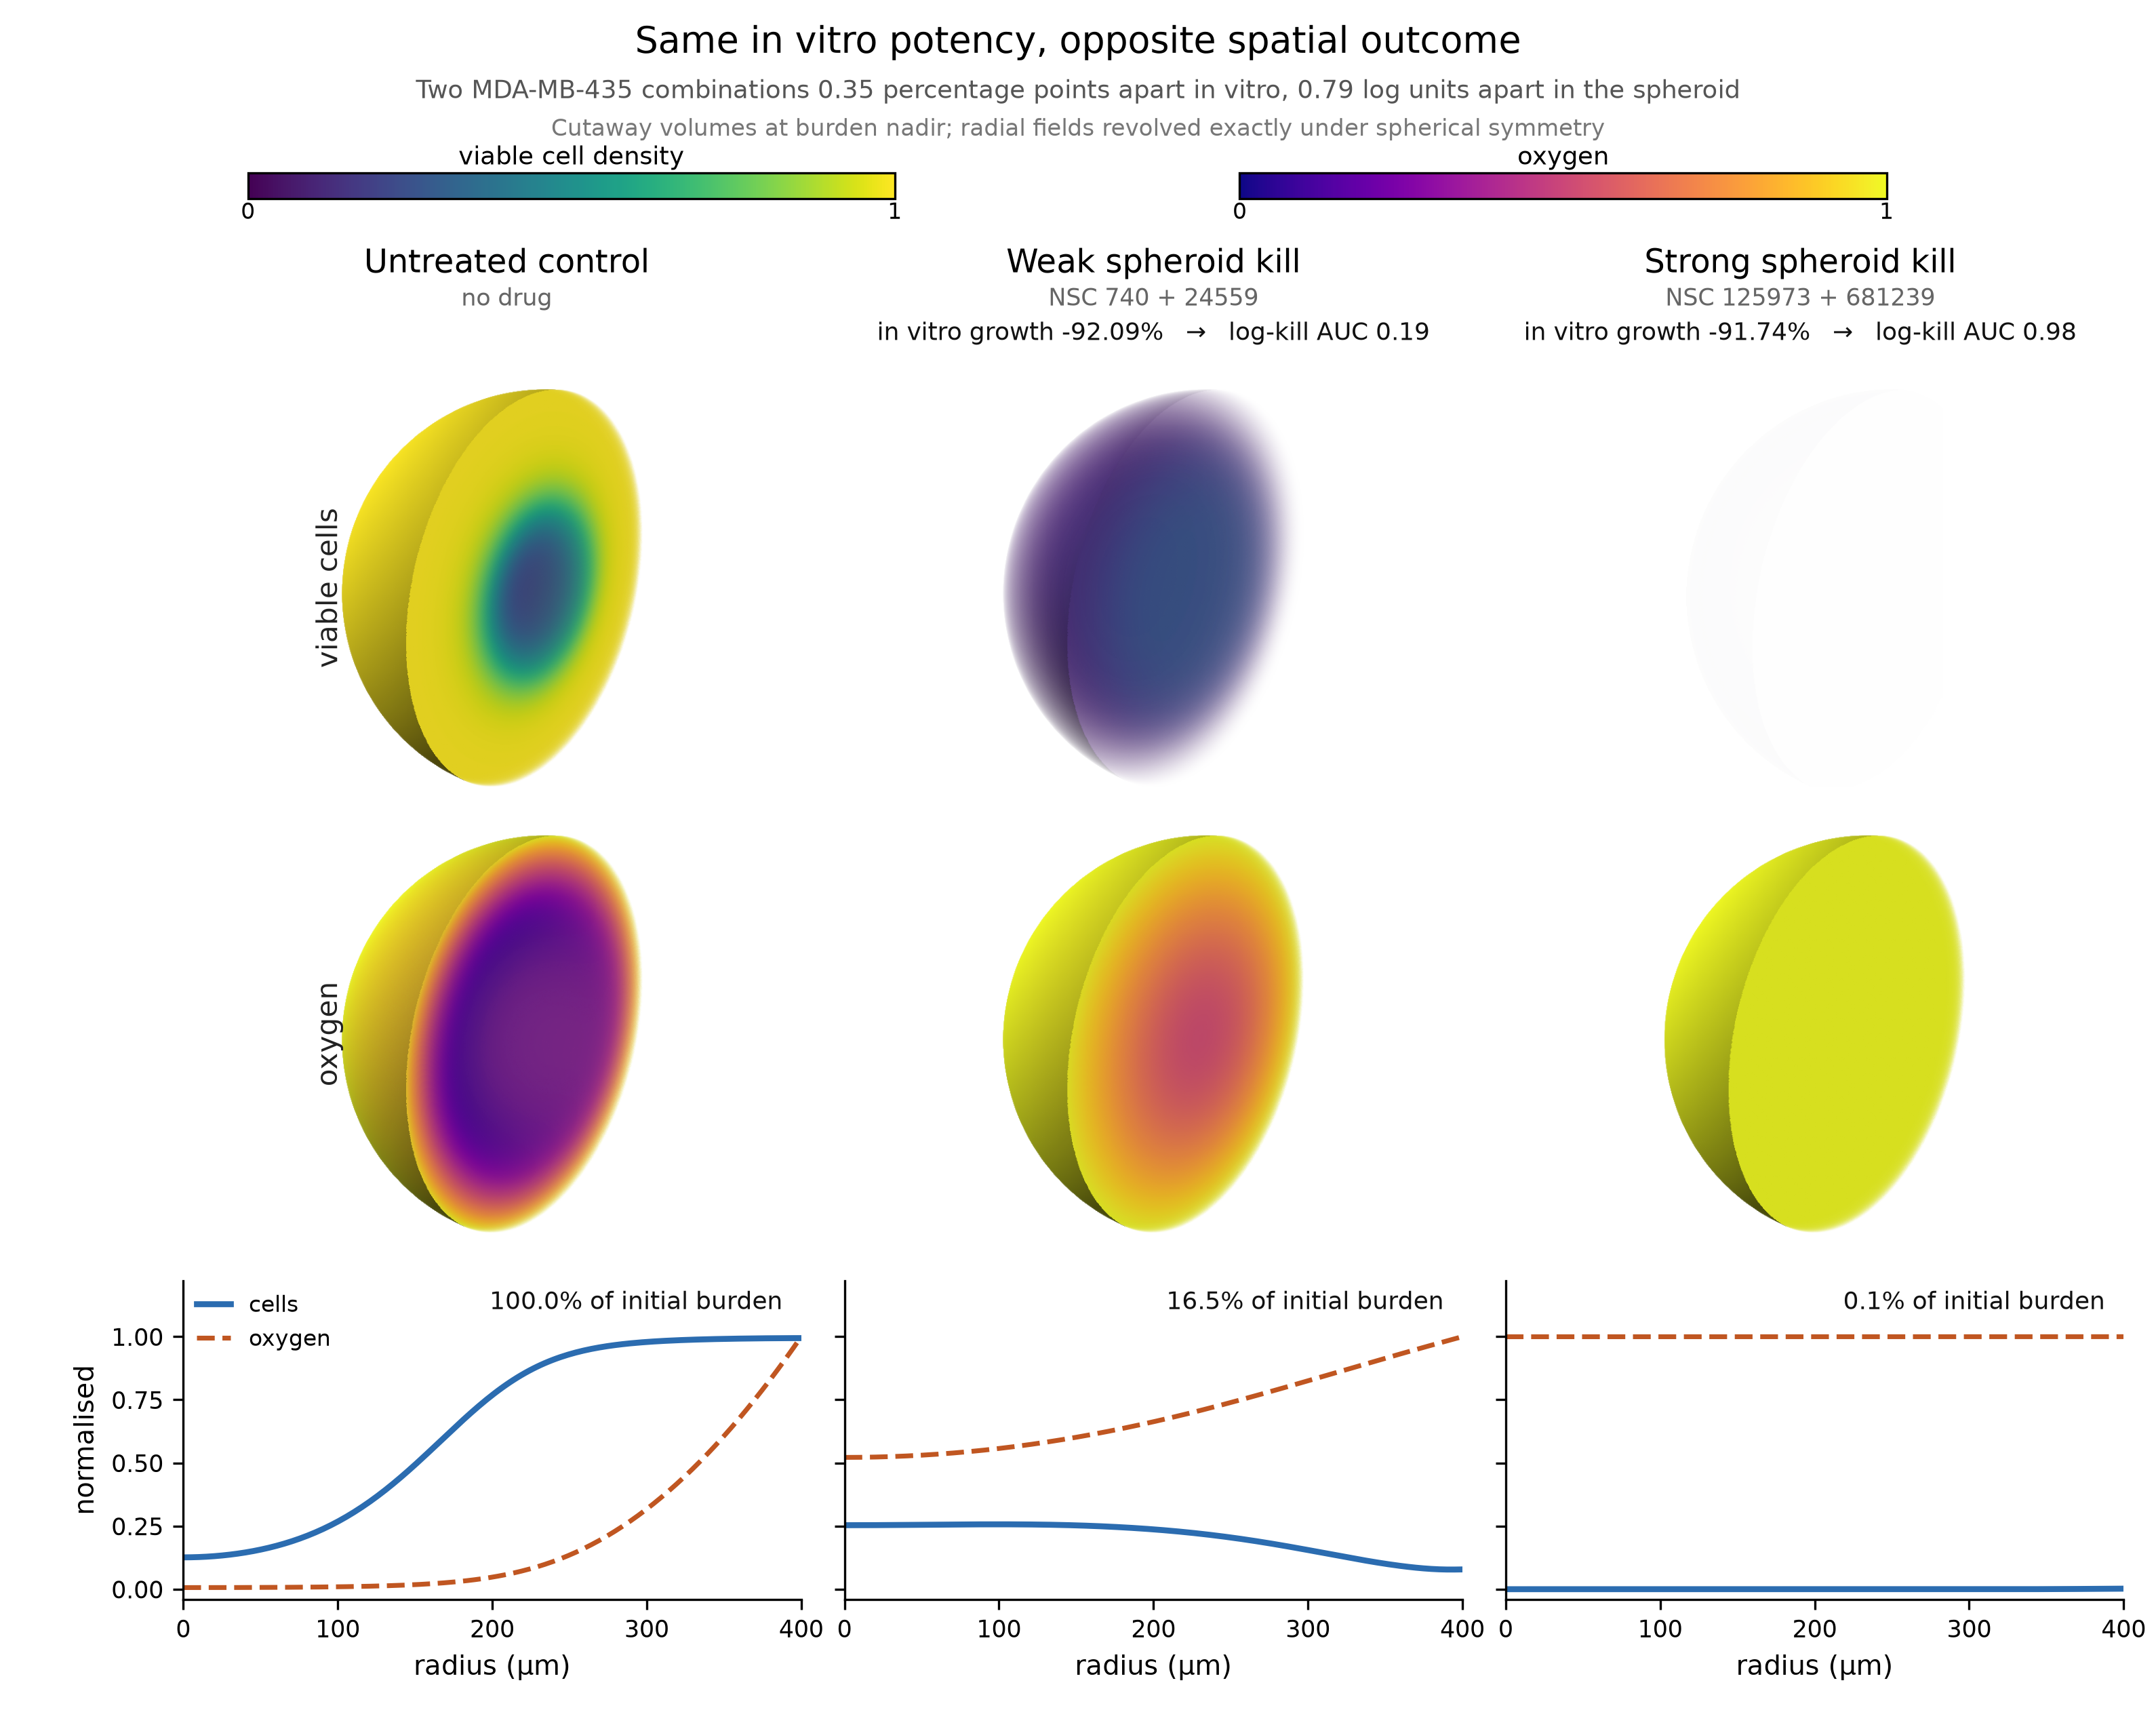
\includegraphics[width=0.80\columnwidth]{figs/fig_spheroid3d.png}
\caption{Volume renderings of the simulated spheroid at burden nadir for two
combinations in MDA-MB-435 that are matched in vitro ($-92.09$ vs $-91.74$
percent growth, $0.35$ points apart) but separated by $0.79$ log units in
the spheroid. Left: viable cell density; right: oxygen. The upper
combination leaves $16.5\%$ of the initial burden behind a spared hypoxic
core; the lower clears to $0.1\%$. Holding assayed potency fixed isolates
the spatial mechanism from drug strength. Rendering integrates the emission--absorption
volume integral over the revolved radial solution, exact for a spherically
symmetric field.}
\label{fig:3d}
\end{figure}

\begin{figure}[t]
\centering
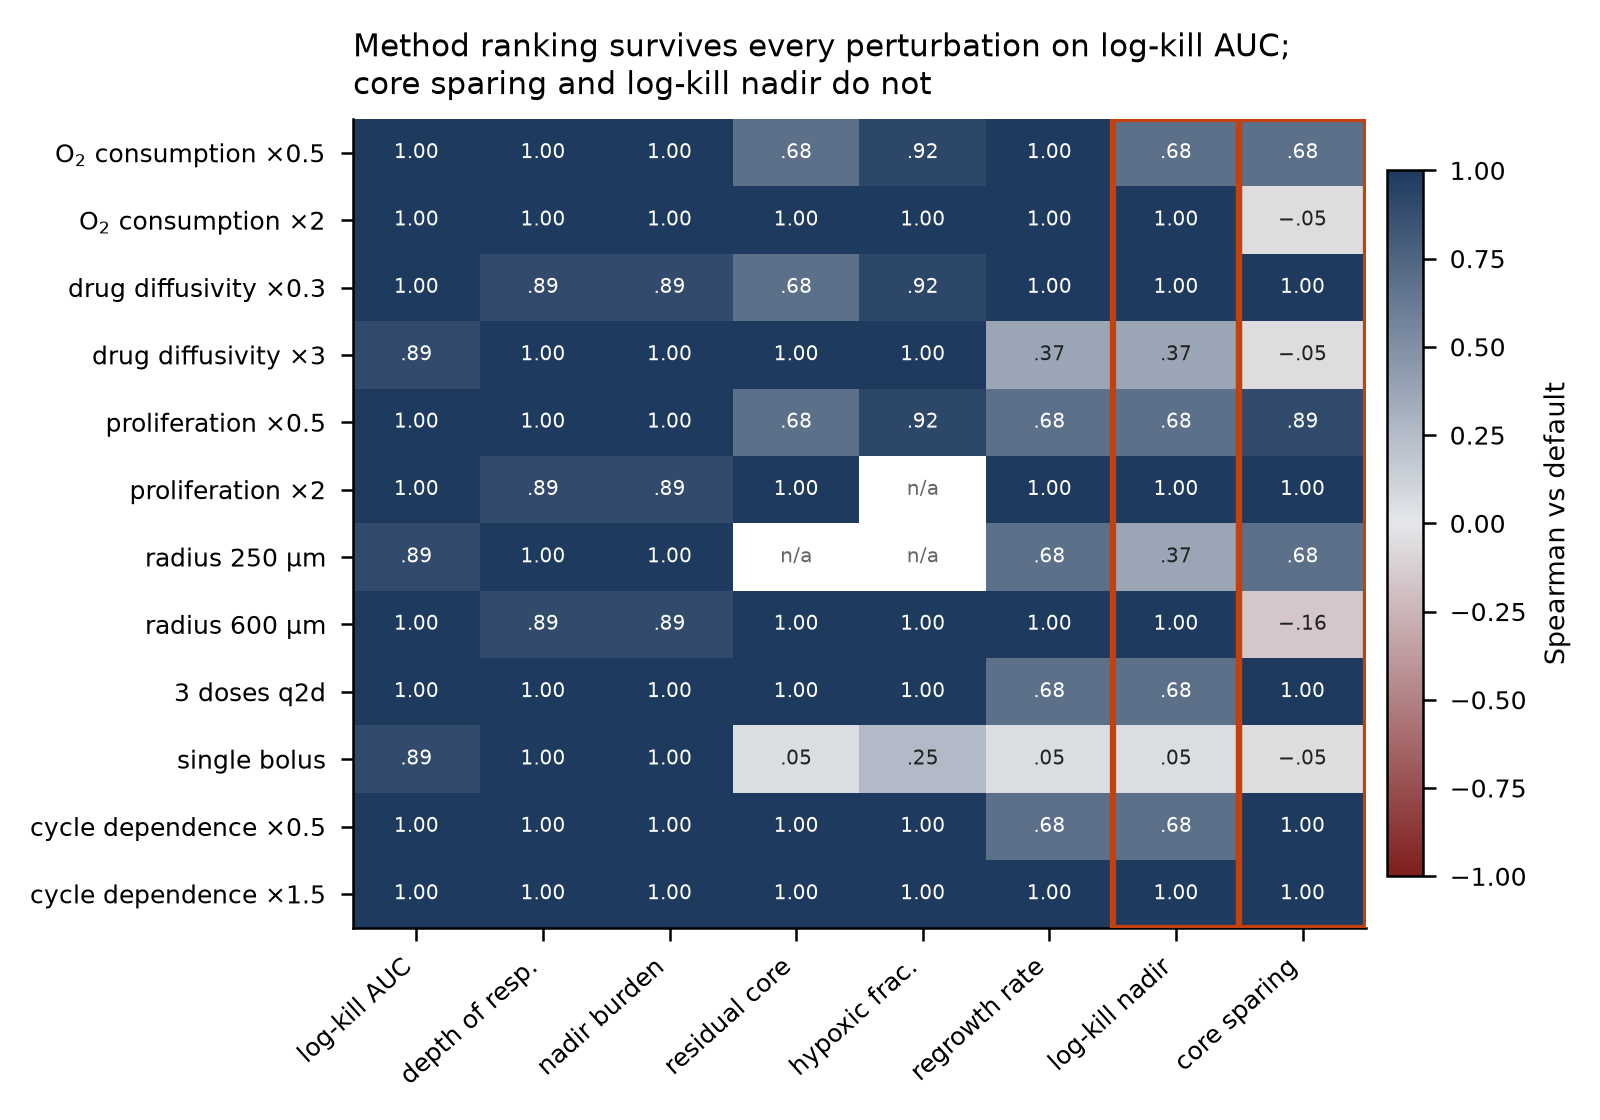
\includegraphics[width=\columnwidth]{figs/fig_robustness.png}
\caption{Robustness of each readout's method ordering across thirteen
parameter perturbations (Spearman against default). Median $\rho = 1.000$;
$\rho \ge 0.8$ in $74.2\%$ of computable cells. Log-kill AUC, which carries
the comparison, never falls below $0.895$. Core sparing and log-kill at nadir
(outlined) are unstable and reported as diagnostics only.}
\label{fig:robust}
\end{figure}

\subsection{Method comparison under a spatial model}
\label{sec:compare}

\cref{tab:methods} ranks all sixteen methods by simulated $K_G$ (the
readout carrying the strongest published survival association) rather than
by the spatial readout; the two orderings agree closely (Spearman
$\rho = -0.86$) and Savitar places fifth under either.

Savitar beats every structural baseline by a wide, highly significant
margin: Tanimoto ($+0.299$ median log-kill AUC, Holm $p < 0.001$), Hamming
and activity-Hamming ($+0.230$), random ($+0.158$), both flat-Mat\'ern
variants, and both of its own ablations. This reproduces the predecessor~\citep{gonehal2026savitar}
paper's finding under a scoring model it was never tuned for. Four
higher-capacity surrogates rank above it, but after Holm correction across
fifteen comparisons only DeepSets does so significantly ($-0.045$ median,
$p = 0.008$); SAASBO ($p = 0.126$), the linear curve baseline ($p = 0.243$)
and deep ensembles ($p = 0.382$) are statistically indistinguishable. On the
spatial readout Savitar places fifth of sixteen (beating ten methods
significantly, tied with four, beaten by one).

\paragraph{The two leaders lead for different reasons.} SAASBO also attains
the best in vitro regret of the sixteen ($7.4$) and the strongest in vitro
potency ($-86.4\%$ growth): its spatial standing follows from solving the
original search problem better, at roughly $600\times$ Savitar's cost
($182$\,s versus $0.3$\,s per BO run at this pool size). DeepSets does not: it ranks fifth on regret, below Savitar, while placing first spatially. \cref{sec:mechanism} separates these cases quantitatively.

\paragraph{A new comparison the predecessor's regime account does not
predict.} That paper evaluates SAASBO only on its chemistry benchmark, never
on the drug panel, so this ALMANAC comparison is run for the first time. Its
account is explicit: SAAS sparsifies which input \emph{dimensions} matter,
Savitar parameterizes which \emph{combinations} interact, so SAAS wins only
on the alloy phase with a small constituent universe. ALMANAC's universe is
large (${\sim}95$ drugs), so that account predicts Savitar should be
favored. It is not: on regret SAASBO wins clearly ($7.40$ vs.\ $14.58$,
better in $51$ of $70$ runs and in all seven cell lines, $p < 10^{-4}$),
while on the spatial readout the two are tied. Which prior wins does not
reduce to constituent-universe size alone.

\paragraph{Dedicated combinatorial-BO methods do not transfer to this pool.}
We additionally run COMBO~\citep{oh2019}, a GP with a diffusion kernel on the graph
Cartesian product of drug identity and ordinal dose, and BOCS, sparse
Bayesian regression over first- and second-order binary indicators, under the
same pool, budget and initialization, with a deviation \emph{favoring}
BOCS, enumerating the finite pool exactly at the acquisition step so it never
loses to an inner-optimizer failure. On three anti-infective screens with
pools of ${\sim}64$--$100$ candidates both are competitive and curve-aware
selection beats them in all six comparisons (margins $0.08$--$4.42$ regret
units, significant in five of six). On ALMANAC, whose enumerated pool is
roughly $700\times$ larger (${\sim}4.7 \times 10^4$ combinations per cell
line), both collapse: mean regret $91.5$ (COMBO) and $78.9$
(BOCS) against $14.6$, worse than random search ($70.4$), and both are beaten
significantly on log-kill AUC ($+0.188$ and $+0.266$ median, Holm
$p < 0.001$) and on $K_G$. Neither consumes the response curve (COMBO sees dose only as an ordinal
level on a path graph, BOCS as a scalar), so at 30 evaluations against the $4{,}000$-candidate subsample every method
scores at each acquisition step (\cref{app:repro}), neither can generalize
across unseen pairs. At small
pool sizes a generic combinatorial prior suffices; at this one it does
not.

\subsection{Mechanism: potency without penetration}
\label{sec:mechanism}

The deficit is mechanistic and legible in the table. Across the sixteen
methods, spheroid performance tracks \emph{residual hypoxic fraction} at
$\rho = -0.969$: more tightly than it tracks in vitro potency
($\rho = -0.767$). Hypoxic fraction is purely spatial: not measurable in a
monolayer, and absent from every method's objective.

To separate ``selects better combinations'' from ``searches better,'' we
regress each method's spatial performance on its in vitro potency and read
the residual: spheroid kill obtained beyond what assayed potency predicts.
This cleanly separates the two leaders. DeepSets is the largest
positive outlier ($+0.140$): it selects combinations that penetrate and
leaves the least hypoxic tissue of any method ($0.091$). SAASBO sits
on the trend line ($+0.014$): it leads spatially because it is the strongest
in vitro searcher, not because it selects better-transporting combinations.
Savitar is the largest negative outlier ($-0.074$): its picks are
\emph{more} potent in vitro than DeepSets' ($-79.2$ vs.\ $-71.7$ percent
growth) yet leave $62\%$ more hypoxic tissue ($0.147$ vs.\ $0.091$).
It converts in vitro potency into spheroid kill less efficiently than any
method in the comparison.

This follows from its design rather than indicating a defect in it. The
curve-aware kernel identifies pairs whose dose--response curves interact
favorably \emph{at the assayed exposure}, which is why it wins on regret.
Nothing in that objective rewards a drug reaching an oxygen-poor core, or
penalizes one whose partner is cycle-dependent and therefore inert in
quiescent tissue. The two tasks overlap heavily but are not the same task.

\paragraph{A shared ceiling.} All sixteen methods are scored on the same
monolayer curves, so this input is constant across the comparison and cannot
itself explain the re-ranking. It does bound what any of them can achieve: an
in vitro curve carries no transport information, and a method optimizing it
perfectly would still be blind to penetration. The re-ranking is caused by
how efficiently each method converts that limited signal into spatial
performance.

\subsection{The out-of-regime cell line}
\label{sec:molt4}

MOLT-4 is reported separately (\cref{tab:molt4}) because it fails the regime
criterion of \cref{sec:cohort}: $6.7\%$ of its pool lies within a small
regret of the optimum, against $0.05\%$ for OVCAR-8. The consequence is visible in the table: every method drives percent growth to $\approx -99$ and regrets compress to under $2$, so the in vitro task carries almost no signal to discriminate on. Four methods tie exactly at the pool optimum.
The spatial readouts still separate them, and the rank agreement between
in vitro and spatial orderings collapses (Kendall $\tau = 0.13$ against
$0.52$ in regime). Pooling MOLT-4 into the main comparison flips three
methods from tied to significantly better than Savitar (SAASBO, the linear
curve baseline and deep ensembles), which is why it is kept separate and
labeled rather than dropped or merged.

\subsection{Robustness}
\label{sec:robust}

A conclusion that holds only at default settings is not a conclusion. Across
thirteen parameter settings perturbing oxygen consumption, diffusivity,
proliferation, radius, schedule and cycle-dependence, the method ordering is
stable in the median (Spearman $\rho = 1.000$ against default; $\rho \ge 0.8$
in $69$ of $93$ computable cells), the curve-aware method ranks first on
log-kill AUC in \emph{all thirteen} settings, and log-kill AUC never falls
below $\rho = 0.895$. Core sparing inverts under four settings and log kill
at nadir has median $\rho = 0.684$, so we report the method comparison as
robust and those two orderings as not established (\cref{app:sweep},
\cref{fig:robust}).

\section{Discussion and Future Work}
\label{sec:future}

The natural reading of these results is not that curve-aware BO is
misconceived, but that it is currently optimizing an objective that stops
short of the phenomenon of interest. Savitar wins decisively on the target it was given, and the target omits transport. What SAAS supplies is a
half-Cauchy prior over per-dimension inverse lengthscales; the curve-aware
kernel uses a single isotropic $\ell$ over $\phi(c)$, treating every
coordinate as a priori equally relevant. The concrete extension is a diagonal
ARD lengthscale under a sparsity-inducing hyperprior, fit by the Type-II step
already in the loop. It is orthogonal to both structural priors (the gate and CP sharing govern how $\phi$ is \emph{built}, the lengthscale prior how it is \emph{compared}), and it targets \cref{sec:mechanism} directly: with transport descriptors appended to the fingerprint, ARD is the mechanism that would let the surrogate discover a transport coordinate matters while most curve coordinates do not. A MAP fit retains the bias without SAASBO's
${\sim}182$\,s NUTS inference. \Cref{app:future} develops this and two
further routes.

\section{Limitations}
\label{sec:limits}

The model is calibrated, not validated: it reproduces spheroid layering and
passes analytic benchmarks (\cref{app:verify}), but no spheroid was grown and
no combination tested, so the claim is comparative (that spatial structure
re-orders selections), not that any absolute number predicts an experiment.
Drug transport is assigned by mechanism class rather than measured;
\cref{app:sweep} bounds the consequence. Readout anchoring is not readout
validation: a simulated $K_G$ is a different quantity from a patient $K_G$,
sharing a name and a functional form. The geometry is radial and avascular: no vasculature, interstitial pressure, immune compartment or resistance evolution. Scope is seven in-regime cell lines plus one
out-of-regime control from a single panel, at one horizon and schedule.

\section{Conclusion}

A well-mixed bridge from in vitro potency to tumor burden is exactly
rank-preserving and cannot change which combination looks better
(\cref{app:ode}); a spatially resolved spheroid can, and does, for $36.5\%$
of pairs. Under that model curve-aware selection keeps a large advantage over
every structural baseline and over two dedicated combinatorial-BO methods,
but falls behind higher-capacity surrogates selecting better-penetrating
combinations. The cause is identifiable: outcome is governed by residual
hypoxic fraction ($\rho = -0.969$), absent from every method's
objective, and points at a fix: a sparsity-aware lengthscale prior over an
interaction-structured feature.


\nocite{*}
\bibliographystyle{icml2025}
\bibliography{refs}

\newpage
\appendix
\onecolumn
\begin{table*}[t]
\caption{Curve-aware selection versus SAASBO on every cell line of the
predecessor paper's~\citep{gonehal2026savitar} ALMANAC set, 10 seeds each. SAASBO attains lower regret
in \emph{all eight} (significantly in three), and higher spheroid log-kill
AUC in six of eight. $p$ is a paired Wilcoxon test, uncorrected.
$^\dagger$MOLT-4 lies outside the published operating regime.}
\label{tab:saas}
\vskip 0.1in
\centering
\small
\setlength{\tabcolsep}{6pt}
\begin{tabular}{lrrrrrr}
\toprule
& \multicolumn{3}{c}{Regret (in vitro)} & \multicolumn{3}{c}{Log-kill AUC (spatial)} \\
\cmidrule(lr){2-4}\cmidrule(lr){5-7}
Cell line & Ours & SAAS & $p$ & Ours & SAAS & $p$ \\
\midrule
MDA-MB-231/ATCC & 13.39 & 0.01 & 0.031 & 0.574 & 0.938 & 0.031 \\
OVCAR-8 & 5.52 & 0.25 & 0.219 & 0.505 & 0.260 & 0.125 \\
MDA-MB-435 & 2.67 & 1.30 & 0.107 & 0.270 & 0.421 & 0.188 \\
T-47D & 5.58 & 1.34 & 0.002 & 0.430 & 0.365 & 0.205 \\
PC-3 & 14.35 & 8.16 & 0.074 & 0.358 & 0.422 & 0.504 \\
HT29 & 21.37 & 17.43 & 0.797 & 0.467 & 0.572 & 0.156 \\
DU-145 & 39.19 & 23.29 & 0.002 & 0.568 & 1.098 & 0.049 \\
MOLT-4$^\dagger$ & 1.09 & 0.41 & 0.129 & 0.458 & 1.566 & 0.004 \\
\bottomrule
\end{tabular}
\end{table*}

\begin{table*}[t]
\caption{MOLT-4, the \textbf{out-of-regime} control, same 16 methods and
ranking. It is excluded from \cref{tab:methods} because $6.7\%$ of its pool
lies within a small regret of the optimum (versus $0.05\%$ for OVCAR-8), so
random search already succeeds, every method drives percent growth to
$\approx -99$, and the in vitro task carries almost no signal to
discriminate on. The spatial readouts still separate the methods, and the
in vitro-to-spatial rank agreement collapses here (Kendall
$\tau = 0.13$ versus $0.52$ in regime).}
\label{tab:molt4}
\vskip 0.1in
\centering
\footnotesize
\setlength{\tabcolsep}{4pt}
\begin{tabular}{lrrrrr}
\toprule
Method & $K_G$ $\downarrow$ & Log-kill & Hypoxic & \%\,growth & Regret \\
\midrule
SAASBO & 0.0052 & 1.566 & 0.004 & -99.5 & 0.41 \\
Linear (curve) & 0.0068 & 1.382 & 0.000 & -99.5 & 0.39 \\
Deep ensemble & 0.0124 & 1.259 & 0.045 & -99.4 & 0.51 \\
DeepSets & 0.0156 & 0.755 & 0.078 & -98.2 & 1.76 \\
Spherical linear & 0.0160 & 1.022 & 0.061 & -99.5 & 0.40 \\
COMBO (graph diffusion) & 0.0190 & 0.904 & 0.097 & -93.9 & 6.00 \\
Mat\'ern (identity) & 0.0191 & 0.930 & 0.085 & -97.8 & 2.09 \\
BOCS (sparse Bayes) & 0.0196 & 0.823 & 0.077 & -95.2 & 4.74 \\
Mat\'ern (curve) & 0.0217 & 0.702 & 0.081 & -97.5 & 2.41 \\
Random & 0.0286 & 0.504 & 0.132 & -96.7 & 3.22 \\
\textbf{Curve-aware (ours)} & 0.0310 & 0.458 & 0.160 & -98.8 & 1.09 \\
Activity-Hamming & 0.0314 & 0.447 & 0.178 & -99.2 & 0.73 \\
Hamming & 0.0314 & 0.447 & 0.178 & -99.2 & 0.73 \\
Ours: no $M$ (ablation) & 0.0314 & 0.447 & 0.178 & -99.2 & 0.73 \\
Tanimoto & 0.0314 & 0.447 & 0.178 & -99.2 & 0.73 \\
Ours: no gate (ablation) & 0.0315 & 0.426 & 0.174 & -99.2 & 0.66 \\
\bottomrule
\end{tabular}
\vskip -0.1in
\end{table*}

\section{Extended Discussion: Toward a Spatially Aware Kernel}
\label{app:future}

\paragraph{The sparsity prior.} What SAAS supplies that the curve-aware
kernel does not is a half-Cauchy prior over per-dimension inverse
lengthscales, letting the surrogate infer that most input coordinates are
irrelevant and concentrate limited evidence on the few that are not. The
curve-aware RBF (\cref{eq:rbf}) uses a single isotropic $\ell$ over
$\phi(c)$: every coordinate is a priori equally relevant. At a
30-evaluation budget this is a real cost, since the curve fingerprint
contributes $p$ parameters per constituent of which typically one or two
carry the signal for a given cell line. The extension is to replace the
isotropic $\ell$ with a diagonal ARD lengthscale
$\ell \in \mathbb{R}^q$ under a sparsity-inducing half-Cauchy hyperprior,
fit by the Type-II marginal-likelihood step already in the loop. This is orthogonal to both structural priors (the activity gate and CP sharing act on how $\phi$ is \emph{built}, the lengthscale prior on how $\phi$ is \emph{compared}), so the two should compose rather than compete. What makes
SAASBO impractical at this pool size is its fully Bayesian NUTS inference
(${\sim}182$\,s per BO run against ${\sim}0.3$\,s); an ARD lengthscale with
a MAP fit retains the inductive bias at a small fraction of that cost.

\paragraph{Three routes.} \emph{Objective augmentation}: score candidates on
a cheap surrogate of penetration (predicted tissue diffusivity and
cycle-dependence from mechanism of action) alongside curve interaction, so
that two combinations of equal assayed potency are no longer equivalent to
the optimizer. \emph{Fingerprint extension}: the per-constituent fingerprint
$e_i$ is already a small parameter vector fit upstream, so appending
transport descriptors requires no change to the kernel algebra; combined
with the ARD prior above it would let the model learn that steep-curve pairs
which are both cycle-dependent are a poor bet in hypoxic tissue.
\emph{Simulation in the loop}: the solver runs ${\sim}1$\,s per combination,
fast enough to serve as the BO objective directly at the ${\sim}30$-evaluation
budgets these campaigns use, turning the spheroid from an evaluation
instrument into the thing being optimized. The comparison also supplies a
target: the spatial deficit is quantified as a residual against the potency
trend, so an extended method can be scored on whether it closes the $0.21$
log-unit gap to DeepSets while retaining its regret advantage.

\begin{figure*}[t]
\centering
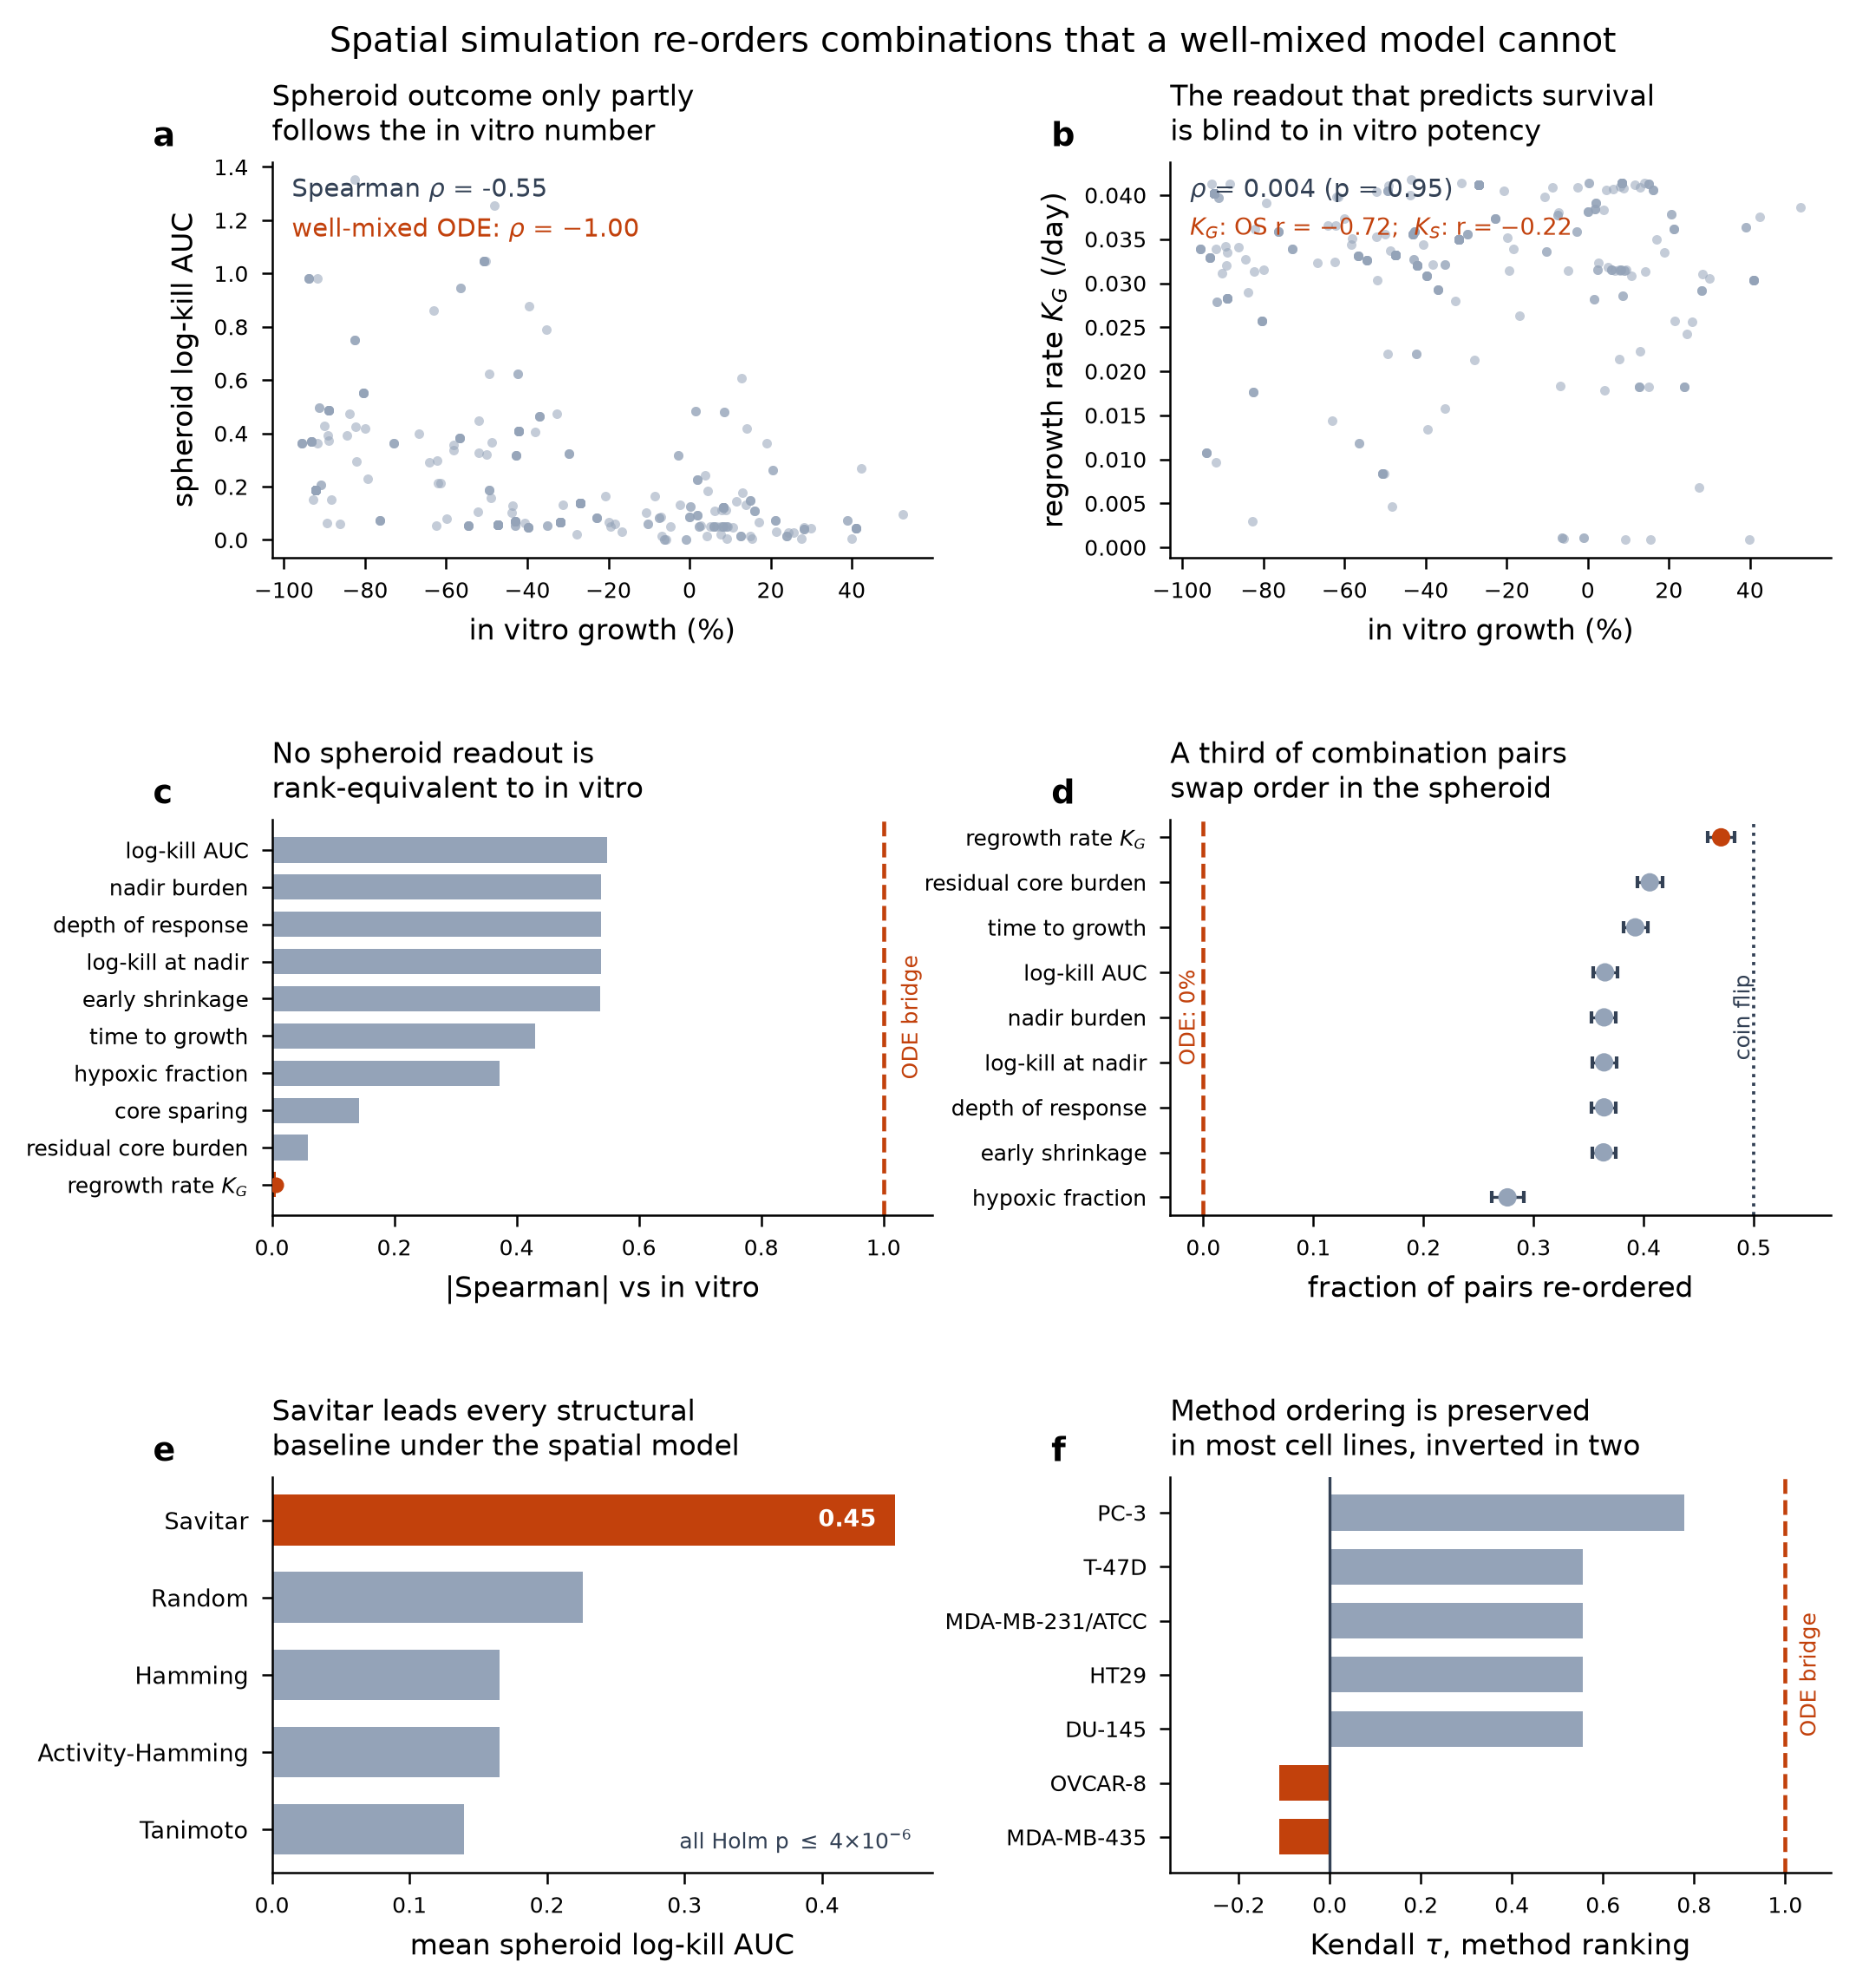
\includegraphics[width=0.80\textwidth]{figs/fig_main.png}
\caption{Spatial simulation re-orders combinations that a well-mixed model
cannot. (a) Spheroid log-kill AUC against the in vitro potency that selected
each combination ($\rho = -0.56$); the well-mixed ODE bridge would place
every point on a monotone curve ($\rho = -1.00$). (b) The clinically
anchored regrowth rate $K_G$ is unrelated to in vitro potency
($\rho = 0.004$, $p = 0.95$), while $K_G$ (not the kill constant
$K_S$) is the quantity that predicts overall survival in patients.
(c) Monotonicity of each readout against in vitro potency. (d) Pairwise
re-ranking rate with bootstrap CIs. (e) Mean log-kill AUC by method.
(f) Per-cell-line rank agreement.}
\label{fig:main}
\end{figure*}

\section{Cross-Combination Generalization}
\label{app:proof}

\begin{theorem}[Cross-combination generalization]
For any combination $c \in \mathcal{C}$ and any constituent $i$ appearing in
$c$, the partial derivative $\partial \phi(c) / \partial A[i,:]$ is non-zero
whenever $|S| \ge 2$ for some $S \subseteq [k]$ containing slot $j$ with
$i_j = i$. Consequently, an observation at any combination $c'$ containing
constituent $i$ propagates information to the posterior predictions at every
other combination $c$ containing $i$, including unseen pairs and triplets.
\end{theorem}

\begin{proof}
Differentiating \cref{eq:cp} yields
$\partial w_S / \partial A[i,r] = \prod_{j' \in S \setminus \{j\}} A[i_{j'}, r]$
whenever some $j \in S$ has $i_j = i$, which is non-zero generically in $A$.
The Gaussian-RBF kernel of \cref{eq:rbf} is a smooth function of $\phi$, so
non-zero gradients of $\phi$ propagate to non-zero gradients of $k(c,c')$ at
any pair sharing constituent $i$.
\end{proof}

\section{Solver Verification}
\label{app:verify}

The radial reaction--diffusion solver is verified against two closed-form
benchmarks before any study result is computed.

\paragraph{Oxygen steady state.} With proliferation disabled, the oxygen field
must relax to the analytic steady state of the spherical diffusion--consumption
equation. Measured relative $L_2$ error: $5.47 \times 10^{-3}$ on the
production mesh.

\paragraph{Fisher--KPP front speed.} With diffusion and logistic growth only,
a travelling front propagates at $c = 2\sqrt{D\rho}$. Seeding a plug at
$r < 6000\,\mu$m in a radius-$12000\,\mu$m domain and fitting only $t > 20$
days (to exclude the transient) gives $169.5$ versus the analytic $178.9$, a
$5.2\%$ error at a mesh ratio of $3.37$. An earlier measurement taken near
the origin during the transient gave a spurious $42\%$ error; the benchmark
must be measured in the travelling-wave regime.

\paragraph{Jacobian banding.} The state is interleaved by node
($[n, O_2, c_1, c_2]$ at $r_0$, then at $r_1$, \ldots) rather than by field,
which makes the Jacobian banded with half-bandwidth $2n_f - 1$. Supplying
\texttt{lband}/\texttt{uband} to the stiff integrator reduces a two-drug
simulation from $298.3$\,s to $2.99$\,s, a $100\times$ speedup with bitwise
identical readouts.

\section{Readout Construction}
\label{app:readouts}

\paragraph{Why time-integrated exposure.} Drug penetration cannot be judged
from a concentration snapshot. With $\tau = R^2/D \approx 3.2$ days against a
$0.25$-day dose, a snapshot at peak surface concentration reports zero or
undefined core penetration for every drug. Measuring the time-integrated
exposure $\mathrm{AUC}(r) = \int c(r,t)\,\mathrm{d}t$ instead separates
transport tiers cleanly: core-to-surface ratio $0.454$ for a slow drug versus
$0.862$ for a fast one.

\paragraph{Why log-kill AUC rather than end-of-horizon log kill.} By day 21
every arm has relaxed toward the same carrying-capacity attractor. The
end-of-horizon log kill spreads only $0.0026$ across all arms; the
time-integrated log-kill AUC spreads $0.0896$ and the log kill at nadir
$0.1118$ (roughly $40\times$ more discriminating). Regional kill fractions
are referenced against the matched untreated control at the same time point
rather than against $t = 0$.

\paragraph{Oxygen consumption is calibrated, not assumed.} The consumption
rate is set so the viable rim of a $400\,\mu$m spheroid falls inside the
$150$--$200\,\mu$m oxygen-diffusion limit: $q = 14$ gives $180.9\,\mu$m and
$q = 16$ gives $164.8\,\mu$m, so we use $q = 15$. With hypoxic death at
$0.25$/day the untreated 21-day spheroid shows a viable rim of $166\,\mu$m,
hypoxic fraction $0.203$ and necrotic fraction $0.058$, reproducing the
layered structure the model is meant to represent.

\section{Reproduction of the Published Pipeline}
\label{app:repro}

Regenerating the ALMANAC combination table from the raw
615\,MB source is bit-identical to the shipped artifact
($2{,}804{,}088/2{,}804{,}088$ rows, max absolute difference $0$). Hill fits
reproduce at Pearson $r = 0.998$--$0.9998$ across parameters, with
$13/6{,}293$ rows ($0.21\%$) differing from optimizer basin flips under a
newer SciPy. BO selections reproduce $138/144$ ($95.8\%$) bit-exactly. A
dedicated re-run of three methods over the analysis cohort matched all
$210/210$ selections on drug identity, percent growth and regret, with
concentration columns agreeing to float round-trip precision
($\le 7.5 \times 10^{-17}$).

\section{The Well-Mixed ODE Control}
\label{app:ode}

The predecessor paper's~\citep{gonehal2026savitar} Gompertz + linear-PK bridge is reimplemented and
validated against its published table. All six rows reproduce, including the
no-treatment row, to a maximum absolute error of $0.0139$ log units (mean
$0.0051$). Applied across $1{,}397$ distinct combinations, the bridge's rank
correlation with in vitro percent growth is Spearman $\rho = -1.0000$
($p = 0$): it is exactly rank-preserving and therefore cannot re-order any
pair of combinations. This is the control against which the spheroid's
$\rho = -0.56$ should be read.

\section{Sensitivity Sweep Detail}
\label{app:sweep}

Thirteen parameter settings perturb oxygen consumption, drug diffusivity,
proliferation rate, spheroid radius, dose schedule and cycle-dependence.
Median Spearman correlation of the method ordering against the default
setting is $1.000$, with $\rho \ge 0.8$ in $69$ of $93$ computable
cells ($74.2\%$; three cells are undefined where a readout is constant).
Per-readout medians: depth of response, log-kill AUC, nadir burden, residual
core burden and hypoxic fraction all exactly $1.000$; regrowth rate $0.842$;
core sparing $0.789$; log kill at nadir $0.684$. The bolus schedule is the
most disruptive single perturbation, degrading five of eight readouts below
$\rho = 0.3$. Core sparing inverts outright under four settings, which is why
it is reported as a mechanistic diagnostic rather than a ranking quantity.

\section{Repository Audit}
\label{app:audit}

An audit of the code released with the predecessor manuscript~\citep{gonehal2026savitar} found the
pipeline reproducible from the shipped intermediates but incomplete at the
edges: the raw NCI-ALMANAC source file and a chemical structure file required
by one baseline are absent (every published NCI download URL now returns
403/404), the shipped ALMANAC results cover 8 cell lines $\times$ 3 seeds
against the manuscript's $60 \times 10$, one results file is misfiled under
the wrong benchmark, and the BO traces record regret without recording the
selected combination, so the selections analysed here had to be recovered
by re-running the loop with the trace extended. None of these contradicts a
published claim; together they mean the headline table cannot be regenerated
from the repository alone.
\end{document}
